\documentclass{beamer}
%Information to be included in the title page:
\title{\textit{Introduction to x86 Assembly}}
\author{Joe Rose}
\institute{GUSEC}
\date{\today}

\usepackage{hyperref}
\hypersetup{
	colorlinks=true,
	linkcolor=blue,    
	urlcolor=blue,
}
\usepackage{tikz}
\usetikzlibrary{shapes,arrows}
\tikzstyle{arrow} = [->,>=stealth]

\useoutertheme{infolines}
\usecolortheme{seagull}
\usefonttheme{professionalfonts}

\logo{
	
\includegraphics[width=1cm]{GUSEC.jpg}
}

\AtBeginSection[]
{
	\begin{frame}
		\frametitle{Outline of the Workshop}
		\tableofcontents[currentsection]
	\end{frame}
}

\tikzstyle{block} = [rectangle, draw, fill=blue!10, 
text width=3cm, text centered, rounded corners, minimum width=3cm, minimum height=1cm]

\tikzstyle{blockhard} = [rectangle, draw, fill=blue!10, 
text width=3cm, text centered, minimum width=3cm, minimum height=1cm]

\begin{document}
	
	\frame{\titlepage}
	
	\begin{frame}{Outline of the Workshop}
		\tableofcontents
	\end{frame}
	
	\section{Introduction}
	\begin{frame}
		\frametitle{Who am I?}
		\begin{itemize}
			\item 3rd Year Comp. Sci. Student
			\item Secretary of GUSEC
			\item Big nerd
		\end{itemize}
	\end{frame}
	
	\section{System Architecture}
	
	\begin{frame}
		\frametitle{Abstraction}

		Modern computer systems can be represented as layers of \textit{abstraction}. As software engineers, we generally work in a 'high level' highly abstracted space, which is then converted by our compiler into low level \textit{machine code}. 

		\begin{center}
			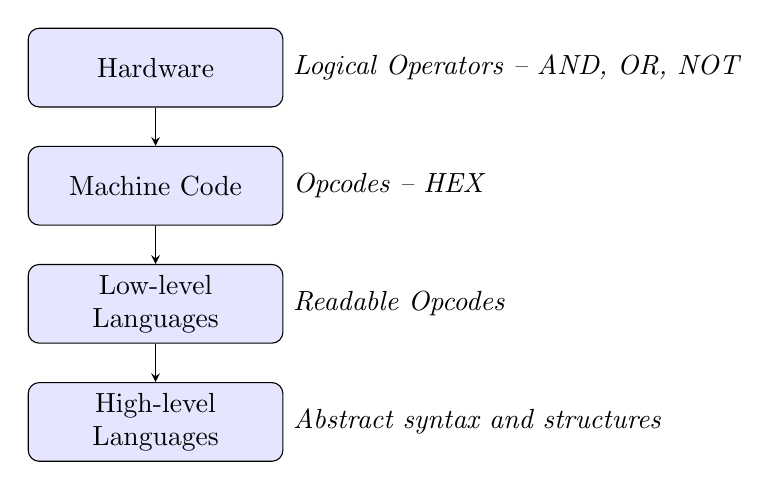
\begin{tikzpicture}[node distance = 1.5cm, auto]
				% Place nodes
				\node (hardware) [block,label=east:\textit{Logical Operators -- AND, OR, NOT}] {Hardware};
				\node (machinecode) [block, label=east:\textit{Opcodes -- HEX}, below of=hardware] {Machine Code};
				\node (lowlevel) [block, label=east:\textit{Readable Opcodes}, below of=machinecode] {Low-level Languages};
				\node (highlevel) [block, label=east:\textit{Abstract syntax and structures}, below of=lowlevel] {High-level Languages};
				
				% Draw arrows
				\draw [arrow] (hardware) -- (machinecode);
				\draw [arrow] (machinecode) -- (lowlevel);
				\draw [arrow] (lowlevel) -- (highlevel);

			\end{tikzpicture}
		\end{center}
	\end{frame}
	
	\begin{frame}
		\frametitle{Memory}
		
		Memory, as it has come to be defined in some current literature, is somewhat of an abstract concept.
		\newline
		
		Every process running at a given time is carved out a little piece of virtual memory. It follows roughly this construction
		
		\begin{center}
			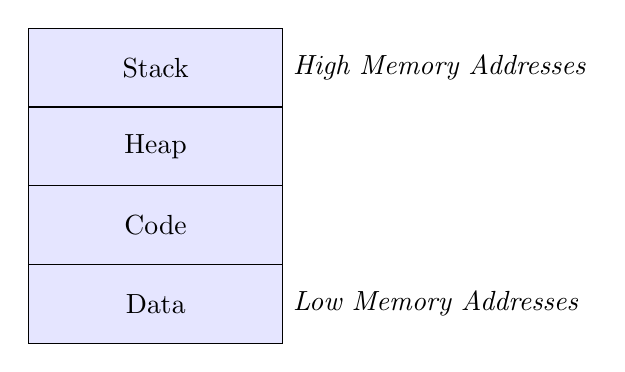
\begin{tikzpicture}[node distance = 1cm, auto]
				% Place nodes
				\node (hardware) [blockhard,label=east:\textit{High Memory Addresses}] {Stack};
				\node (machinecode) [blockhard, below of=hardware] {Heap};
				\node (lowlevel) [blockhard, below of=machinecode] {Code};
				\node (highlevel) [blockhard, label=east:\textit{Low Memory Addresses}, below of=lowlevel] {Data};
				
				
			\end{tikzpicture}
		\end{center}	
	\end{frame}
	
	\section{x86}
	
	\begin{frame}
		\frametitle{The Registers}
		
		In low-level languages we deal with the regsiters. Registers are extremely small (32-bit) pieces of memory within your CPU which are quicker than RAM or cache to access. These are what store the pieces of data currently being worked with. The x86 specifies some general purpose registers and some dedicated registers. 
		\newline
		
		\begin{tabular}{|c|l|}
			\hline
			\textbf{Register} & \textbf{Purpose} \\
			\hline
			\hline
			EAX & Accumulator\\
			\hline
			ECX & Counter in loops\\
			\hline
			ESI & Source in string \& memory operations\\
			\hline
			EDI & Destination in string \& memory operations\\
			\hline
			EBP & Stack base pointer\\
			\hline
			ESP & Stack Pointer\\
			\hline
		\end{tabular}
	\end{frame}
	
	
	
	\section{Finishing Off}
	
	\begin{frame}
		\frametitle{Sources}
		
		These are the books I got the content for this workshop from. However, there is a huge amount of free literature on x86 and these are by no means necessary for you to learn the ropes. 
		\newline		
		
		\begin{itemize}
			\item \href{https://www.worldcat.org/search?q=bn:9781593274306}{\textit{Practical Malware Analysis} - Chapter 4. A Crash Course in x86 Disassembly}
			\item \href{https://www.worldcat.org/search?q=bn:9781593274306}{\textit{Practical Reverse Engineering} - Chapter 1. x86 and x64}
			\item \href{https://www.wiley.com/en-gb/Practical+Reverse+Engineering:+x86,+x64,+ARM,+Windows+Kernel,+Reversing+Tools,+and+Obfuscation-p-9781118787311}{\textit{Practical Binary Analysis} - Appendix A. A Crash Course in x86 Disassembly}
		\end{itemize}		
	\end{frame}
	
	
\end{document}